\documentclass[a4paper,12pt,twoside,french]{book}
\usepackage[
    %backend=biber, 
    natbib=true,
    style=numeric,
    sorting=none     
]{biblatex}
\addbibresource{biblio.bib}%Import the bibliography file

\usepackage[french]{babel}
\usepackage[utf8]{inputenc}
\usepackage[T1]{fontenc}
\usepackage[a4paper,left=3cm,right=2.5cm,top=3cm,bottom=3cm, twoside]{geometry}
\usepackage{xcolor}
\usepackage{stmaryrd}
\usepackage{amssymb}
\usepackage{amsmath}
\usepackage{libertine}
\usepackage[pdftex]{graphicx}
\usepackage{caption}
\usepackage{subcaption}
\usepackage{float}
\usepackage{multirow}
\usepackage{apalike}
\usepackage{minitoc}
\usepackage{tikz}
\usepackage{enumitem}
\usepackage{epigraph}
%\usetikzlibrary{shadows.blur}
\usepackage{lscape}
\usepackage{titletoc}
%\usepackage{lipsum}
%\usepackage{cite}
\usepackage{booktabs}
\usepackage{arydshln}
\usepackage[nonumberlist]{glossaries}
\usepackage{calc}
\usepackage[]{titlesec} 
\definecolor{linkColor}{HTML}{32a852}
\usepackage[colorlinks=true,citecolor=linkColor,linkcolor=black]{hyperref}
\usepackage{fancyhdr}
\usepackage{lipsum}

\usepackage{setspace}
\onehalfspacing

%%%%%%%%%%%%%%%%%%%%%%%%%%%%%%%%%%%%%%%%%%%%%%%%%%%%%%%%%%%%%%%%%%%%%%%%%%
%%%%%%%%%%%%%%%%%%%%%%%%%%%%%%%%%%%%%%%%%%%%%%%%%%%%%%%%%%%%%%%%%%%%%%%%%%

\definecolor{yourcolor}{HTML}{8a0e19}%{008bb2}

\titleformat{\chapter}[display]
{\normalfont\color{yourcolor}}
{\filleft\huge\color{black}\textsc\chaptertitlename\hspace*{2mm}%
	\begin{tikzpicture}[baseline={([yshift=-.6ex]current bounding box.center)}]
	\node[fill=yourcolor,circle,text=white] {\thechapter};
	\end{tikzpicture}
}
{1ex}
{\titlerule[1.5pt]\vspace*{1.5ex}\Huge\color{black}\textsc}
[]

\titleformat{name=\chapter,numberless}[display]
{\normalfont\color{black}}
{}
{1ex}
{\vspace*{-5cm}\Huge\textsc}
[]

%command to print the acutal minitoc
\newcommand{\printmyminitoc}[1]{%
	\noindent\hspace{1cm}%
	\colorlet{chpnumbercolor}{black}%
	\begin{tikzpicture}
	\node(s){
		\begin{minipage}{.9\linewidth}%minipage trick
		\printcontents[chapters]{}{1}{}
		\end{minipage}
	};
	{
		\color{yourcolor}
		\draw(s.north west)--(s.north east) (s.south west)--(s.south east);
	}
	\end{tikzpicture}
	\vspace*{3ex}
	
	#1
	\vfill
	\pagebreak
}


\newcommand{\HRule}{\rule{\linewidth}{0.7mm}}
\newcommand{\Hrule}{\rule{\linewidth}{0.3mm}}

%%%%%%%%%%%%%%%%%%%%%%%%%%%%%%%%%%%%%%%%%%%%%%%%%%%%%%%%%%%%%%%%%%%%%%%%%%%%%
%%%%%%%%%%%%%%%%%%%%%%%%%%%%%%%%%%%%%%%%%%%%%%%%%%%%%%%%%%%%%%%%%%%%%%%%%%





\begin{document}
	
%\maketitle
%----------------------------------------------------------------------------------------
%	TITLE PAGE
%----------------------------------------------------------------------------------------
	\begin{titlepage}
		\begin{center}
			\begin{tabular}{c@{\hskip 7cm}c@{\hskip 1cm}}
				
\includegraphics[height=2.5cm]{UParisCitelogo.jpg} &
				%si autre logo : \includegraphics[height=2.3cm]{figures/PageTitre/logo_ic_2021.jpg}
			\end{tabular}
		\end{center}
	
		\begin{center}
		
\vspace*{.03\textheight}
\textsc{\LARGE Université Paris Cité}\\[0.2cm] % Univ name
		\large 	ISIFAR \\ 
        %Équipe de recherche\\
  
  			\vfill
 
	 		\rule{\textwidth}{0.8pt} \\ % Horizontal line
	 		\vspace{10pt}
	 		 { \LARGE \bfseries Estimation du nombre de cluster à l'aide du Gap Statistique} % Thesis title
	 		 \vspace{10pt}
	 		 \rule{\textwidth}{0.8pt} \\ % Horizontal line
		\end{center}
		
		\vfill
		% Author and supervisor	
		\begin{center}
			Par\\ \textsc{\Large Steve BASSO NGOUNE \\  Ruoqi ZHU \\ \vspace{8pt}Hengze WANG}\\[1cm] 
            
			Projet Master en \textsc{\large Apprentissage Statistique}\\[1.2cm]
            
		
            \vspace{1cm}
	
			Novembre 2024
		\end{center}
        		\vspace{1cm}
			
		
		\begin{center}
			\begin{tabular}{lll}
				\textsc{Aurélie Fischer} & Professeur \\
				
			\end{tabular}\\[1cm]
		\end{center}
		
		\vspace{1cm}

	\newpage %page de garde vide
	\thispagestyle{empty} %page de garde vide
	\end{titlepage}


\pagestyle{fancy}

\fancyhead{}

\renewcommand{\chaptermark}[1]{\markboth{\textsc{#1}}{}}


\frontmatter

\tableofcontents
\addcontentsline{toc}{chapter}{Table des matières}

% \listoffigures
% \addcontentsline{toc}{chapter}{Liste des figures}

% \listoftables
% \addcontentsline{toc}{chapter}{Liste des tableaux}


\mainmatter

\setlength{\parskip}{.7em}

\titlespacing*{\section}{0pt}{.9em}{.8em}
\renewcommand{\baselinestretch}{1.1}


\fancyhead[RO]{\leftmark}
\fancyhead[LE]{\textsc{\chaptername~\thechapter}}


\chapter*{Introduction}
%\startcontents[chapters]
\addcontentsline{toc}{chapter}{Introduction}  


Dans le domaine de l'analyse de clustering, déterminer le nombre optimal de clusters représente un défi de taille. Le Gap Statistic\cite{tibshirani_estimating_2001}, ou "statistique de l’écart", est une méthode d’évaluation cruciale qui a émergé pour répondre à ce besoin. Son principe repose sur la comparaison entre la structure de clustering des données réelles et celle d'une distribution de référence pour déterminer le nombre de clusters le plus approprié. Cette méthode fournit un moyen systématique et quantitatif d’évaluer la pertinence des résultats de clustering.

Le calcul du Gap Statistique implique plusieurs étapes clés. Tout d'abord, pour un jeu de données donné et différents nombres hypothétiques de clusters, on calcule la variance intra-cluster, mesurant ainsi la cohésion des points au sein de chaque cluster. Une variance faible indique une similarité élevée entre les points d'un même cluster. Ensuite, une distribution de référence est construite, généralement par des méthodes de randomisation ou de simulation. On calcule ensuite la variance intra-cluster attendue dans cette distribution de référence. Enfin, on évalue la qualité des résultats de clustering pour chaque nombre de clusters en calculant la valeur du "Gap", soit la différence entre la variance intra-cluster réelle et celle attendue dans la référence. Un Gap élevé indique que la structure de clustering réelle se distingue de manière significative de la structure attendue sous la distribution de référence, suggérant que le nombre de clusters choisi est approprié.

Le Gap Statistique présente de nombreux avantages. Il ne dépend pas d'hypothèses spécifiques sur la distribution des données, ce qui lui confère une grande polyvalence pour traiter divers types de données. Comparé aux règles empiriques traditionnelles ou aux méthodes de jugement subjectif, le Gap Statistic fournit un critère d'évaluation objectif basé sur des principes statistiques, réduisant ainsi les biais humains. Dans la pratique, cette méthode a été largement adoptée dans plusieurs domaines. Par exemple, en recherche biomédicale, elle aide les chercheurs à analyser les données d'expression génétique pour identifier des sous-types de maladies potentiels ou des biomarqueurs ; en études de marché, elle permet de segmenter les groupes de consommateurs, facilitant ainsi l’élaboration de stratégies de marketing plus ciblées. Le Gap Statistique constitue donc une méthode précieuse pour déterminer le nombre optimal de clusters en analyse de clustering.

Le but de cette étude est de comprendre le fonctionnement de la méthode, puis de l'appliquer à des données simulées avant de la tester sur une base de données réelle.




%\part{Stae of the art}
\chapter{Aspect Théorique}

Dans la littérature, de nombreuses méthodes ont été utilisées pour déterminer le nombre de clusters optimaux. Parmi celles ci, nous pouvons citer:

\subsection*{La méthode de Milligan et Cooper (1985)}

La méthode de Milligan et Cooper (1985) consiste à maximisée suivant les valeurs de k l'indice suivant:
\[
CH(k)=\frac{B(k)/(k - 1)}{W(k)/(n - k)}
\]

Ou, où \(B(k)\) et \(W(k)\) sont respectivement la somme des carrés entre les groupes et la somme des carrés intra-groupes pour \(k\) groupes. Le nombre de clusters est donc donner par la valeur k qui maximise \(CH(k)\)

\subsection*{La méthode de  Krzanowski et Lai (1985)}

En se basant sur les travaux de Marriott (1971),Krzanowski et Lai (1985) proposent pour trouver le nombre de cluster optimal de maximiser la quantité \(KL(k)\) donnée par:

\[
KL(k)=\left|\frac{DIFF(k)}{DIFF(k + 1)}\right|
\]
Ou,
\[
DIFF(k)=(k - 1)^{2 / p}W_{k - 1}-k^{2 / p}W_{k}
\]

Le nombre de cluster est donc donné par la valeur de \(k\) qui maximise \(KL(k)\)

\subsection*{La méthode de Kaufman et Rousseeuw (1990)}

Kaufman et Rousseeuw (1990) proposent d'utiliser le coefficient de silhouette. Et de prendre la valeur de \(k\) qui maximise la moyenne des valeurs de \(s(i)\) pour l'ensemble des données . Pour une observation \(i\), \(s(i)\) est donné par:
\[
s(i)=\frac{b(i)-a(i)}{\max \{a(i), b(i)\}}
\]
Ou, \(a(i)\) la distance moyenne à d'autres points dans son groupe et \(b(i)\) la distance moyenne à tous les points du groupe le plus proche en dehors de son propre groupe

Il ressort donc que la plupart des méthodes présentes dans la littérature ne sont pas valables pour \(k=1\), autrement dit, elle ne permettent pas de dire s'il est possible ou non de faire un clustering. Robert Tibshirani et al.(2000) ont mis sur pied la méthode du Gap Statistique qui permet non seulement de déterminer le nombre de clusters optimale, mais aussi de tester s'il est nécessaire ou pas de créer des clusters.

\section{Gap Statistics}

Nos données ${x_{ij}}$ (où $i = 1, 2, ..., n$ et $j = 1, 2, ..., p$) sont constituées de $n$ observations indépendantes mesurées sur $p$ caractéristiques. Soit $d_{ii'}$ la distance entre les observations $i$ et $i'$. Le choix le plus courant pour $d_{ii'}$ est la distance euclidienne au carré :
$$
\sum_{j} (x_{ij} - x_{i'j})^{2}
$$
Supposons que nous avons regroupé les données en $k$ clusters $C_{1}, C_{2}, \ldots, C_{k}$, où $C_{r}$ représente les indices des observations dans le cluster $r$, et $n_{r} = \vert C_{r} \vert$.Soit
$$
D_{r}=\sum_{i, i' \in C_{r}} d_{i i'} \
$$ 
la somme des distances entre toutes les paires de points dans le cluster $r$, et définissons
$$
W_{k}=\sum_{r=1}^{k} \frac{1}{2 n_{r}} D_{r} \ (2)
$$
Tout d'abord, $D_{r} = \sum_{i, i' \in C_{r}} d_{ii'}$, qui représente la somme des distances entre toutes les paires de points dans le cluster $r$.
Ensuite, $W_{k} = \sum_{r = 1}^{k} \frac{1}{2n_{r}} D_{r}$, soit la somme, pour chaque cluster $r$ (avec $r$ variant de $1$ à $k$), du produit de $D_{r}$ par $\frac{1}{2n_{r}}$. Ici, $n_{r}$ est le nombre d'observations dans le cluster $r$ ($n_{r} = |C_{r}|$).
Lorsque la distance $d$ est la distance euclidienne au carré, $W_{k}$ représente la somme des carrés des distances intra-clusters autour des moyennes de chaque cluster, où le coefficient $2$ assure la cohérence de ce calcul. Dans cette notation, la taille de l’échantillon $n$ est omise. En général, plus la valeur de $W_{k}$ est petite, plus les points au sein des clusters sont rapprochés, ce qui indique potentiellement une meilleure qualité de clustering. Cette mesure est utilisée pour évaluer la qualité du clustering en fonction du nombre de clusters $k$ et joue un rôle important dans le calcul de la statistique de l’écart (Gap Statistic) dans les étapes ultérieures.

Prenons deux exemples simples. Considérons un cluster $r$, où $D_r$ représente la somme des distances entre toutes les paires de trois observations dans ce cluster. Supposons simplement que la distance entre chaque paire de points est la même, afin de simplifier la compréhension. Étant donné que chaque distance entre deux points est comptée deux fois (par exemple, la distance entre le point $i$ et le point $i'$, ainsi que celle entre $i'$ et $i$), cela équivaut à deux fois la somme des longueurs des arêtes.
\begin{figure}[H]
    \centering
    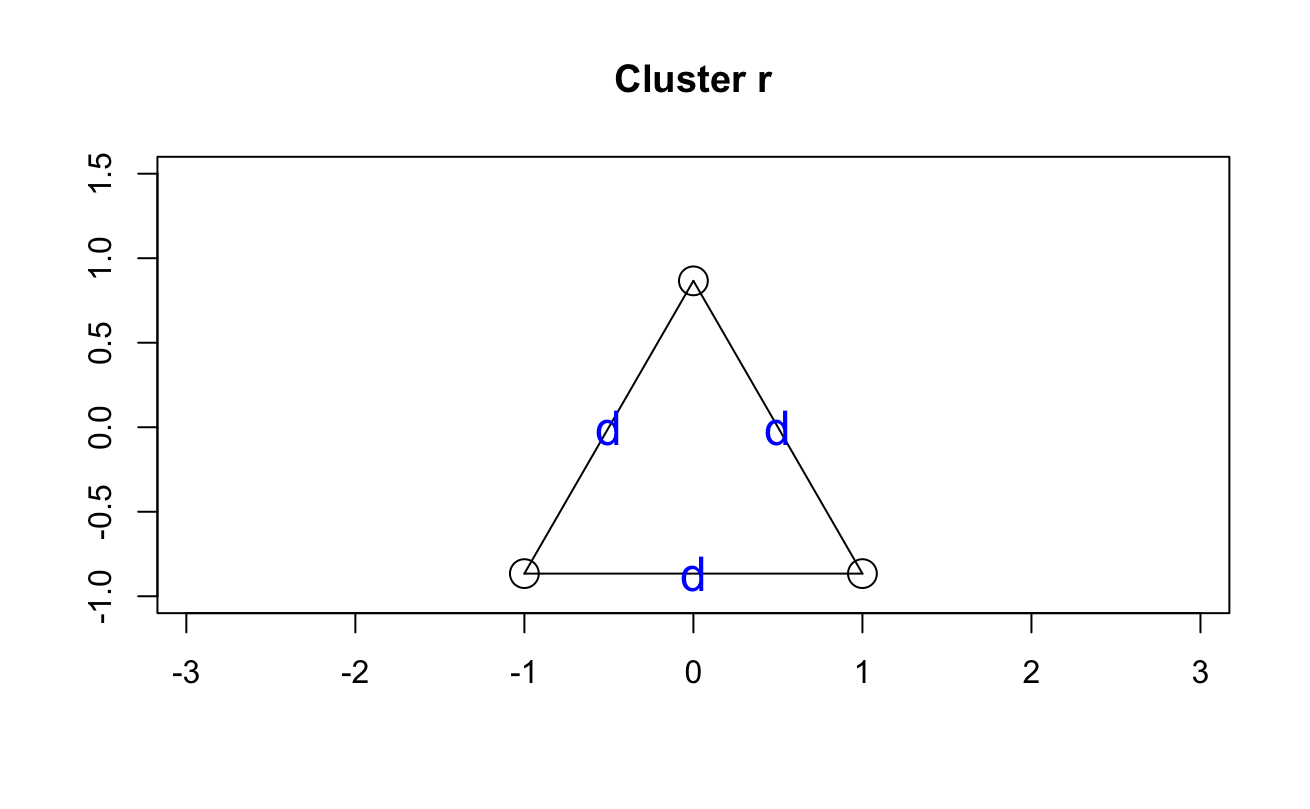
\includegraphics[width=1\linewidth]{images/cluster r.png}
    \caption{Exemple K = 1}
    \label{fig:enter-label}
\end{figure}

$$
D_r = D \times 2 \times 3
$$

Prenons un autre exemple pour $W_k$ où $k = 3$.
\begin{figure}[H]
    \centering
    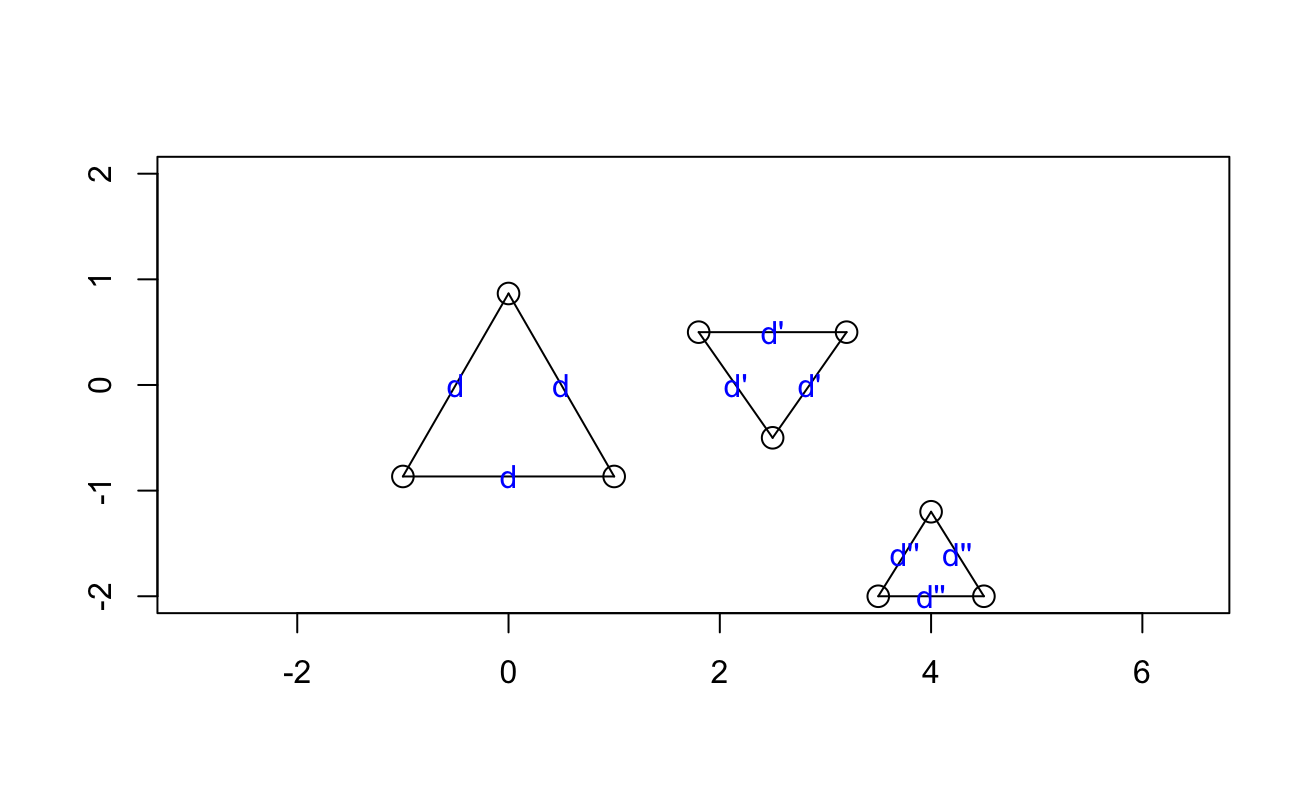
\includegraphics[width=0.9\linewidth]{images/3triangles.png}
    \caption{Exemple K = 3}
    \label{fig:enter-label}
\end{figure}
$$
W_k = \sum_{r=1}^{k = 3} \frac{D_r}{2 n_r} =\frac{ d \times 2 \times 3 + d' \times 2 \times 3 + d'' \times 2 \times 3}{2\times3}
$$

\begin{figure}[H]
    \centering
    % 左侧图片
    \begin{subfigure}[b]{0.45\linewidth}
        \centering
        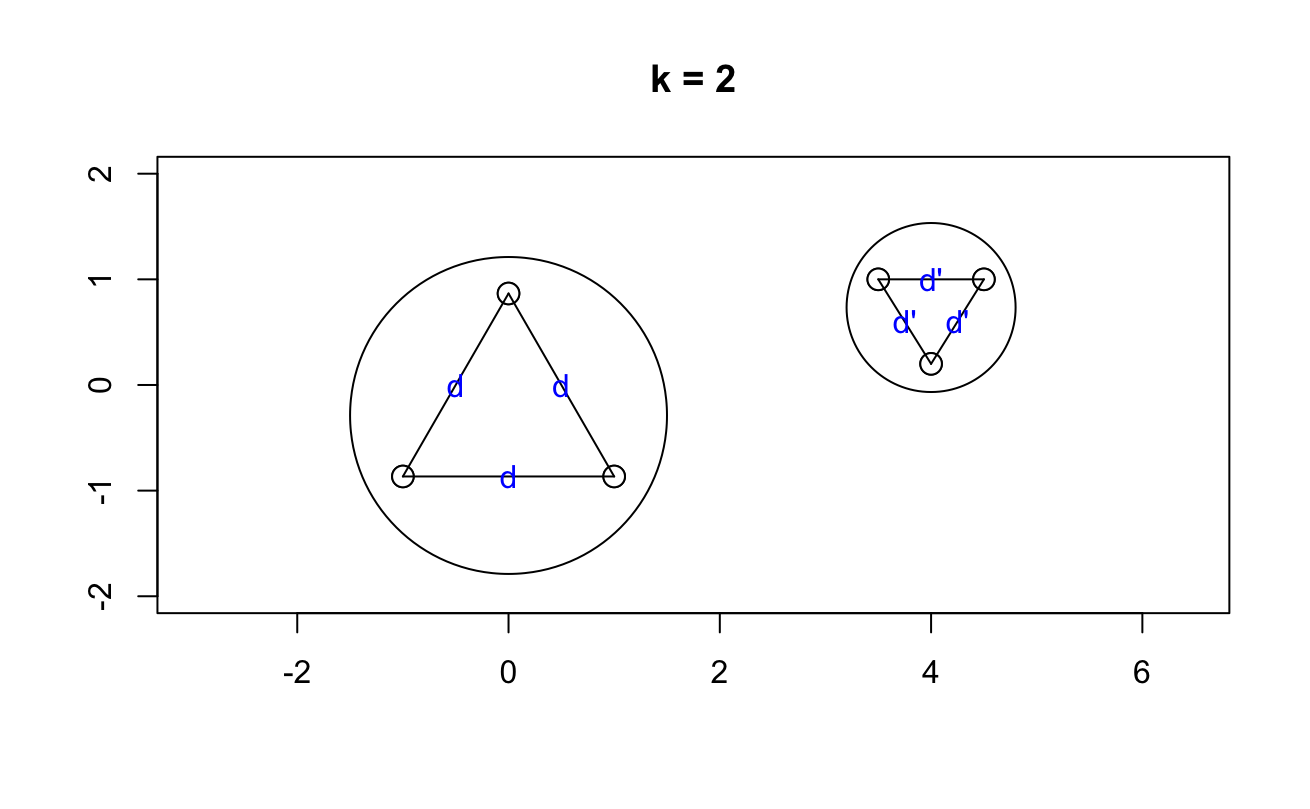
\includegraphics[width=\linewidth]{images/2k.png}
        \caption{K = 2}
        \label{fig:2k}
    \end{subfigure}
    \hspace{0.05\linewidth} % 两张图片之间的间隔
    % 右侧图片
    \begin{subfigure}[b]{0.45\linewidth}
        \centering
        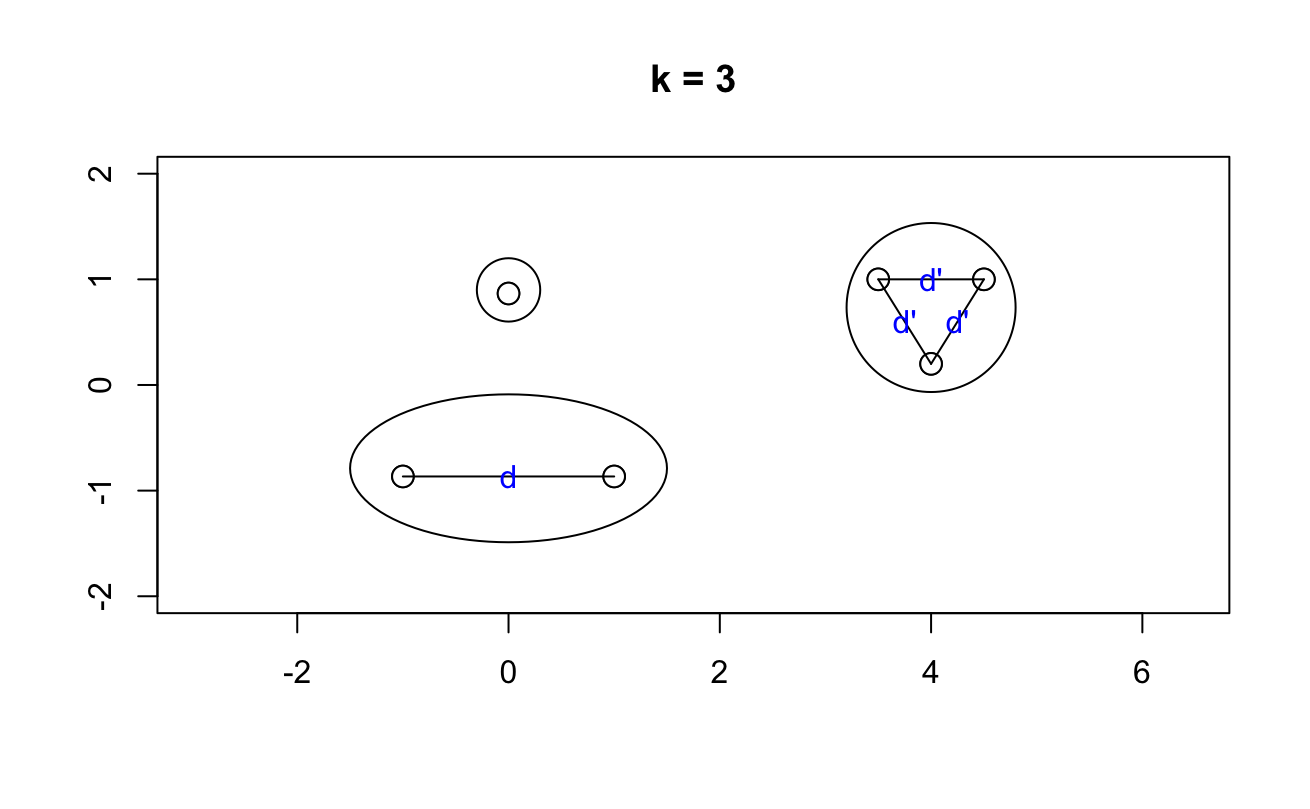
\includegraphics[width=\linewidth]{images/3k.png}
        \caption{K = 3}
        \label{fig:3k}
    \end{subfigure}
    
    \caption{}
    \label{fig:side-by-side}
\end{figure}

Dans cet exemple simple, si le nombre de clusters dépasse 2 à 3, alors la distance moyenne $W_k$ reste inchangée.
$$
\begin{aligned}
W_2 &= \sum_{r=1}^{2} \frac{D_r}{2 n_r} =\frac{ d \times 2 \times 3 + d' \times 2 \times 3}{2\times3} = d+d'\\
 W_3 &=\sum_{r=1}^{3} \frac{D_r}{2 n_r} =0+ \frac{d \times 2 \times 2}{2 \times 2 }+\frac{d' \times 2 \times 3 }{2 \times 3 } = d+d'
\end{aligned}
\Longrightarrow W_2 = W_3
$$

En comparant le graphique de $\log (W_{k})$ avec la valeur attendue des données sous une distribution de référence appropriée pour l'hypothèse nulle, on peut ainsi le standardiser.Ensuite, notre estimation du nombre optimal de clusters est la valeur de $k$ pour laquelle la diminution de $\log (W_{k})$ par rapport à cette courbe de référence est la plus importante.

Par conséquent, nous définissons , pour chaque $k \in \mathbb{N_*}$:

$$
Gap_{n}(k) = E_{n}^{*}\left\{\log \left(W_{k}\right)\right\}-\log \left(W_{k}\right) \ (3) 
$$


\begin{figure}[H]
    \centering
    % 第一排图片
    \begin{subfigure}[b]{0.45\linewidth} % 左侧子图
        \centering
        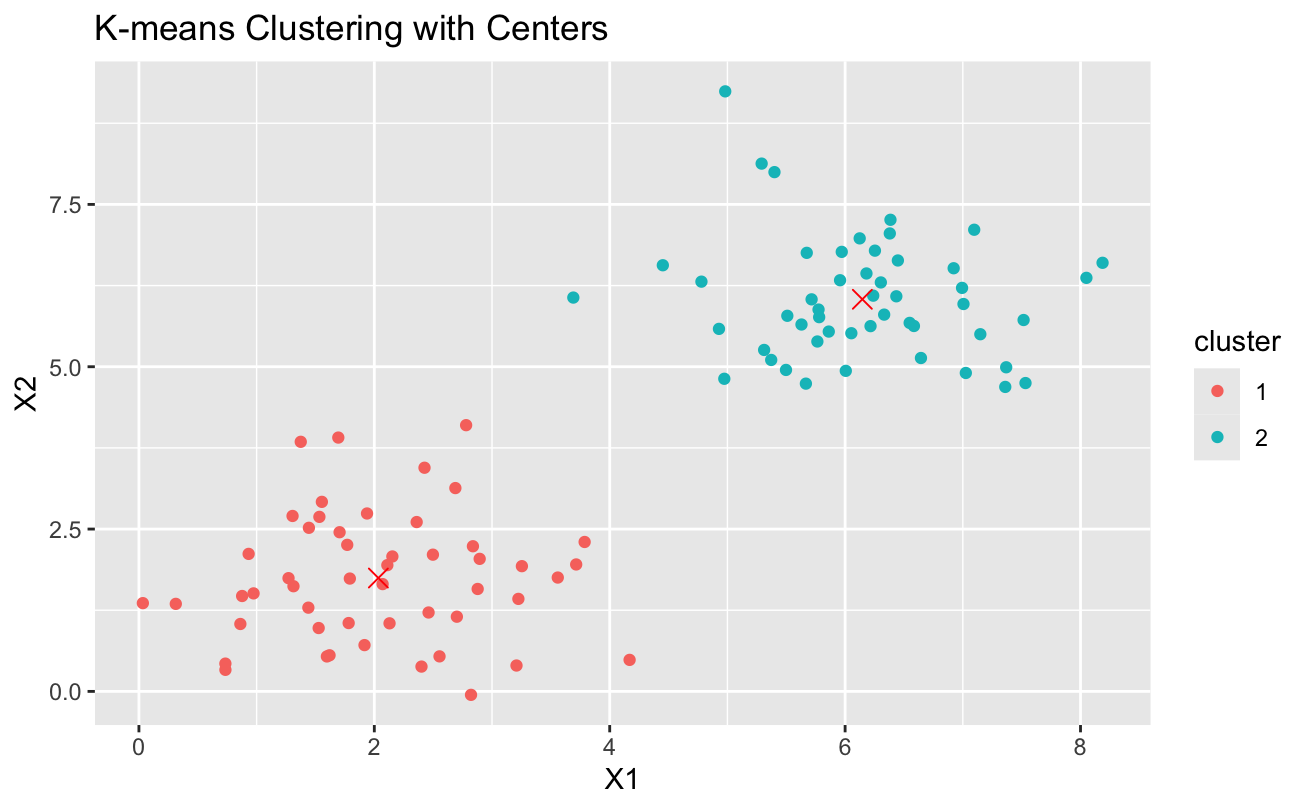
\includegraphics[width=\linewidth]{images/A.png}
        \caption{Nuage}
        \label{fig:image-A}
    \end{subfigure}
    \hspace{0.05\linewidth} % 两个子图之间的间隔
    \begin{subfigure}[b]{0.45\linewidth} % 右侧子图
        \centering
        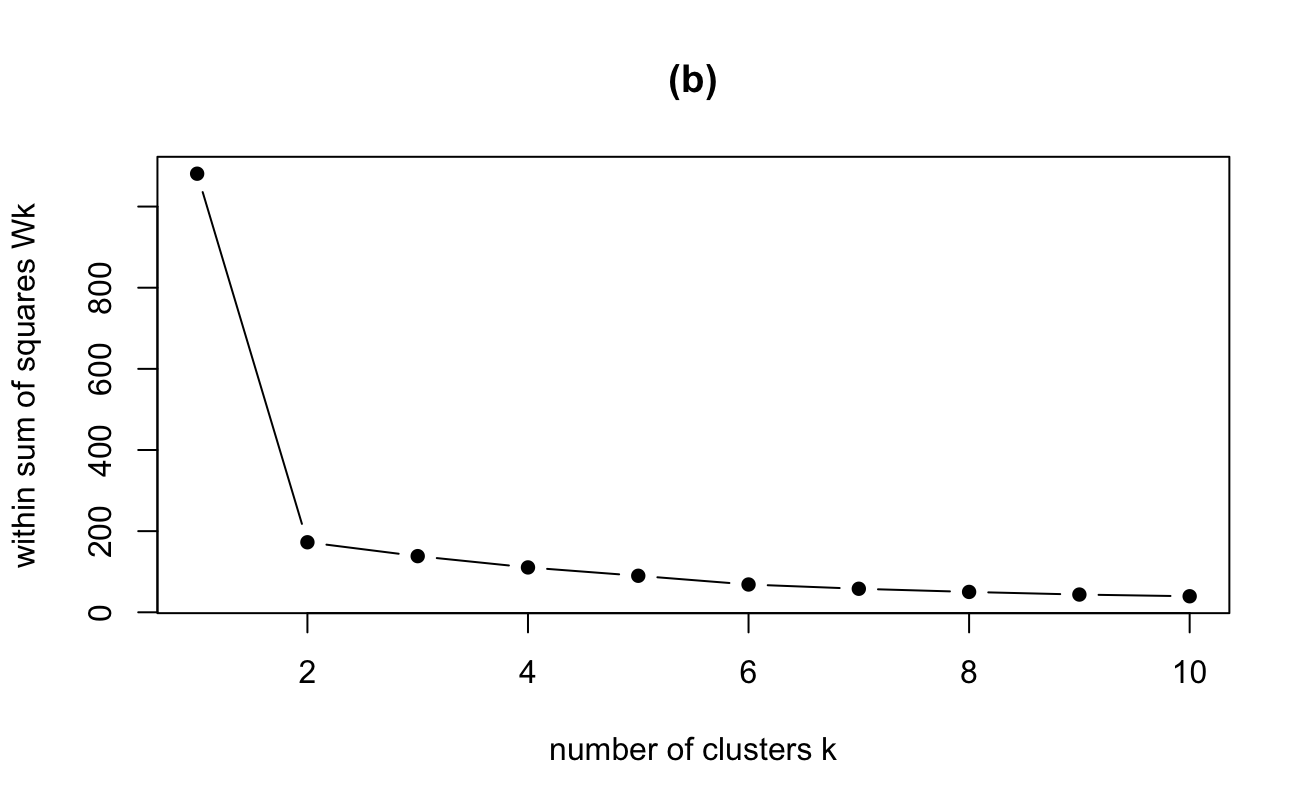
\includegraphics[width=\linewidth]{images/B.png}
        \caption{$W_k$}
        \label{fig:image-B}
    \end{subfigure}
    
    % 第二排图片
    \vspace{0.5cm} % 第一排和第二排之间的间隔
    \begin{subfigure}[b]{0.45\linewidth} % 左侧子图
        \centering
        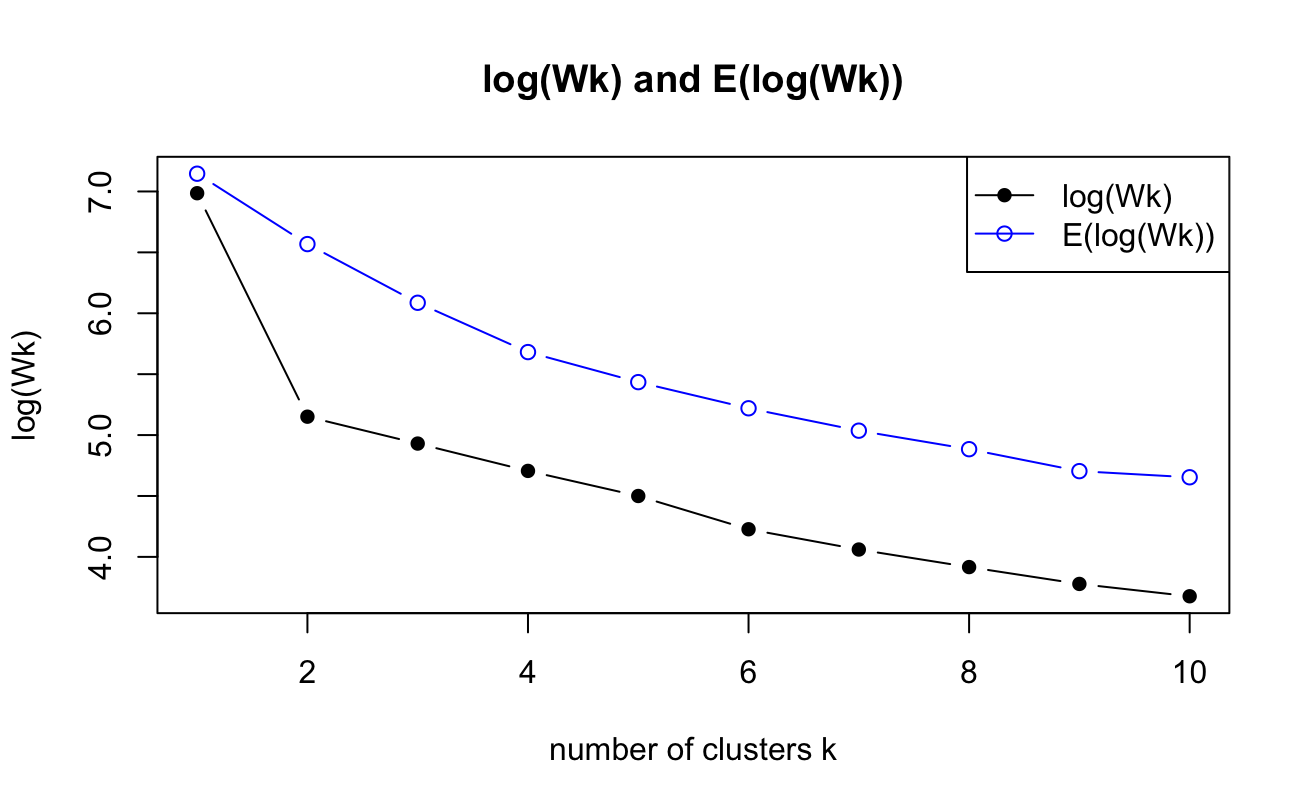
\includegraphics[width=\linewidth]{images/C.png}
        \caption{Espérence et logarithme}
        \label{fig:image-C}
    \end{subfigure}
    \hspace{0.05\linewidth} % 两个子图之间的间隔
    \begin{subfigure}[b]{0.45\linewidth} % 右侧子图
        \centering
        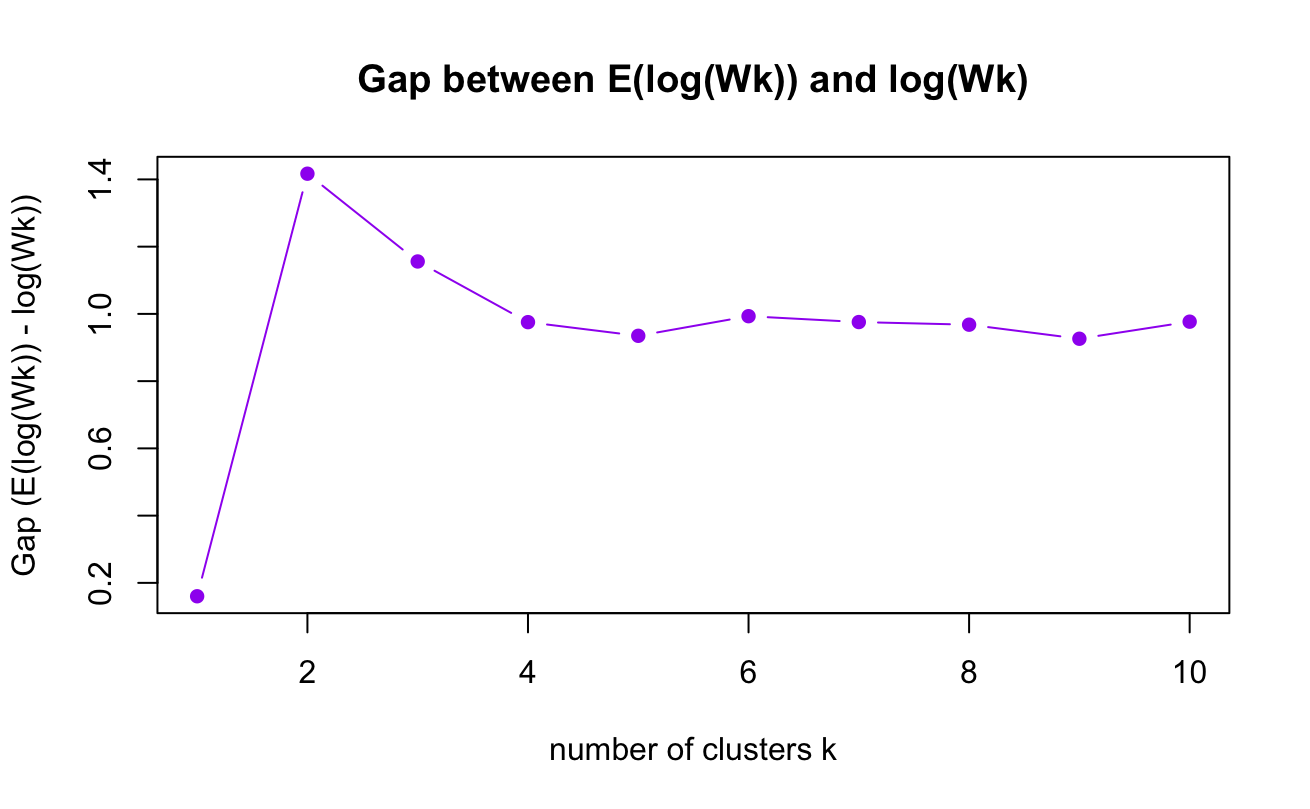
\includegraphics[width=\linewidth]{images/D.png}
        \caption{Le Gap}
        \label{fig:image-D}
    \end{subfigure}
    
    \caption{}
    \label{fig:four-images}
\end{figure}

\section{Reference distribution}

Pour transformer le Gap Statistic en procédure opérationnelle, nous devons trouver une distribution de référence appropriée et évaluer la distribution d'échantillonnage du Gap Statistic.

\subsection{Principe de génération}

Nous supposons que le dataset d'échantillons est $X$, avec $n$ samples, $p$ features.

$$
\text{X} = 
\begin{bmatrix}
  & x_{1,1} & \cdots & \cdots & x_{1,p} \\
  & \vdots & \ddots &  \ddots &\vdots \\
  & x_{i,1} & \cdots  & \cdots & x_{i,p} \\
  & \vdots & \ddots  & \ddots & \vdots \\
  & x_{n,1} & \ddots & \cdots & x_{n,p} \\
\end{bmatrix}
\text{n samples, p features}
$$

Pour chaque feature, il doit y avoir une valeur minimale et une valeur maximale. Par exemple, la première feature : $X_1 \in [x_{1,min},x_{1,max}]$.

Générons de manière aléatoire d'une distribution de référence par une distribution continue uniforme, nous obtenons :

$$
\text{$X'_1$} = 
\begin{bmatrix}
  & x'_{1,1} \\
  & \vdots  \\
  & \vdots \\
  & x'_{n,1} \\
\end{bmatrix}
\text{n samples}
$$ 

où $x'_{i,1} \in [x_{1,min},x_{1,max}]$.

Pour les autres features, nous les générons de la même manière, alors nous obtenons la distribution de référence $X'$ :

$$
\text{X'} = 
\begin{bmatrix}
  & x'_{1,1} & \cdots & \cdots & x'_{1,p} \\
  & \vdots & \ddots &  \ddots &\vdots \\
  & x'_{i,1} & \cdots  & \cdots & x'_{i,p} \\
  & \vdots & \ddots  & \ddots & \vdots \\
  & x'_{n,1} & \ddots & \cdots & x'_{n,p} \\
\end{bmatrix}
\text{n samples, p features}
$$

Nous désignons par $S^{p}$ l'ensemble de ces distributions à composante unique (ou variables aléatoires) sur $R^{p}$.

Pour voir comment trouver une distribution de référence appropriée, considérons un instant la version de la population correspondant au Gap Statistic dans le cas du regroupement par K-means :
$$
g(k)=\log\left\{\frac{MSE_{X^{*}}(k)}{MSE_{X^{*}}(1)}\right\}-\log\left\{\frac{MSE_{X}(k)}{MSE_{X}(1)}\right\}
$$ où $MSE_{X}(k)=E(\min_{\mu\in A_{k}}\|X - \mu\|^{2})$.

Le gap statistic compare les performances du modèle null (un cluster) à celles des modèles alternatifs ($k > 1$) en mesurant la réduction de la variance intra-cluster. $A_{k}\subset R^{p}$ est un ensemble de $k$-points minimisant cette variance. La statistique est normalisée pour que $g(1)=0$, facilitant la comparaison entre le modèle nul et les modèles avec plusieurs clusters.

Selon l'article, nous introduisons maintenant deux théorèmes sur la distribution de référence.

Pour des lois univarié, la distribution de référence est donnée par le théorème suivant:

\textbf{Théorème 1}. Soit \(p = 1\). Alors, pour tous \(k \geq 1\).

\begin{equation}
\inf_{X \in S^p} \left\{ \frac{MSE_{X}(k)}{MSE_{X}(1)} \right\} = \frac{MSE_{U}(k)}{MSE_{U}(1)}
\end{equation}

Ou , \(S^{p}\) représente l'ensemble des distributions (ou variables aléatoires) à une seule composante dans \(R^{p}\).

Ce théorème montre que, dans le cas univarié, la distribution de référence est donnée par la loi uniforme \(U = U[0,1]\). 

Dans le cas multidimensionnel, déterminer la loi de référence n'est plus aussi simple comme le montre le résultat suivant:

\textbf{Théorème 2}. Si \(p > 1\), alors,aucune distribution \(U \in S^{p}\) dont le  support est différent d'une droite, ne peut satisfaire l'équation (1).
Pour $p>1$, il n'existe aucune distribution de référence $U \in S^{p}$, sauf si son support est réduit à un sous-ensemble dégénéré (ex. une ligne droite).

Donc, en dimensions élevées, on ne peut pas utiliser une méthode générique pour comparer les modèles. Cela limite l'applicabilité directe du Gap Statistic telle qu'elle est définie pour les cas univariés.

Une solution consiste à générer des données de référence à partir de l'estimateur du maximum de vraisemblance (MLE) sous contrainte de log-concavité.

En dimension 1, cette estimation peut être réalisée à l'aide d'algorithmes d'approximation convexes.

On constate alors que dans le cas multidimensionnelle, on est pas capable de trouver directement la distribution de référence. Robert \textit{Tibshirani et al.(2000)} en se basant sur le théorème 1 proposent donc d'utiliser une méthode numérique basée sur la \textit{simulation de Monté Carlo}.


\subsection{Méthode Numérique pour l'estimation de de la distribution de référence}

\begin{enumerate}[label=(\alph*)] % Définit le style de numérotation
	\item Pour chaque caractéristique de référence, générer des valeurs pour cette caractéristique de manière uniforme dans la plage des valeurs observées pour cette caractéristique.
	
	\item Générer les caractéristiques de référence à partir d'une distribution uniforme dans un rectangle aligné avec les composantes principales des données. Plus précisément, si \(X\) est notre matrice de données de dimension \(n \times p\), supposons que les moyennes des colonnes sont égales à \(0\) et calculons la décomposition en valeurs singulières : 
	\[
	X = UDV^{T}.
	\]
	Nous effectuons une transformation : 
	\[
	X' = XV,
	\]
	puis, comme dans la méthode (a), nous tirons des caractéristiques uniformes \(Z'\) dans la plage des valeurs des colonnes de \(X'\). Enfin, nous effectuons une transformation inverse : 
	\[
	Z = Z'V^{T},
	\]
	pour obtenir les données de référence \(Z\)
\end{enumerate}

La méthode (a) a l'avantage de la simplicité. La méthode (b) prend en compte la forme de la distribution des données et, tant que la méthode d'agrégation elle-même est invariante, peut rendre l'ensemble du processus invariant par rotation.

Dans chaque cas, nous estimons \(E_{n}^{*}\{\log (W_{k})\}\) en prenant la moyenne de \(B\) copies de \(\log (W_{k}^{*})\), où chaque \(\log (W_{k}^{*})\) est calculé à partir d'un échantillon de Monte Carlo $X_{1}^{*}, \ldots, X_{n}^{*}$ tiré de notre distribution de référence. Enfin, nous devons évaluer la distribution d'échantillonnage de la statistique d'écart. Soit \(sd(k)\) l'écart type de \(B\) répétitions de Monte Carlo des \(\log (W_{k}^{*})\). En outre, compte tenu de l'erreur de simulation dans \(E_{n}^{*}\{\log (W_{k})\}\), nous obtenons la quantité
\[
s_{k}=\sqrt{(1 + 1 / B)} sd(k)
\]

\subsection{Algorithme pour le choix du nombre de cluster}
La procédure est la suivante:

\textbf{Étape 1} : Effectuer une agrégation des données d'observation en faisant varier le nombre total de groupes de \(k = 1\), \(2\), \(\ldots\), \(K\), afin d'obtenir les valeurs de la mesure de dispersion intra-groupe \(W_{k}\) (où \(k = 1\), \(2\), \(\ldots\), \(K\)).

\textbf{Étape 2} : Utiliser l'un des deux choix de distribution uniforme mentionnés ci-dessuspour générer \(B\) ensembles de données de référence et effectuer une agrégation pour chacun de ces ensembles de données de référence, afin d'obtenir les valeurs de la mesure de dispersion intra-groupe \(W_{k b}^{*}\) (où \(b = 1\), \(2\), \(\ldots\), \(B\), \(k = 1\), \(2\), \(\ldots\), \(K\)). Calculer la statistique d'écart (estimée)
\[
Gap(k)=\frac{1}{B}\sum_{b}\log\left(W_{k b}^{*}\right)-\log\left(W_{k}\right)
\]

\textbf{Étape 3} : Soit \(\tilde{I}=\frac{1}{B}\sum_{b}\log (W_{k b}^{*})\), calculer l'écart type
\[
sd_{k}=\left[\frac{1}{B}\sum_{b}\left\{\log (W_{k b}^{*}) - \overline{I}\right\}^{2}\right]^{\frac{1}{2}}
\]

En utilisant cette condition, nous choisissons la taille du groupe \(k\) comme étant la plus petite valeur de \(k\) qui satisfait \(Gap(k) \geq Gap(k + 1) - s_{k + 1}\)
% Ajoutez d'autres sections ici si nécessaire





%\part{Contribution}
\chapter{Implémentation De la méthode du Gap Statistique}

\startcontents[Implémentation]

\section{Implémentation De la méthode du Gap Statistique}

Dans cette partie, nous allons utiliser et comparer la performance du Gap Statistique aux autres méthodes. Nous allons dans un premier temps l'appliquer sur des données simulées et dans un second temps sur des données réelles.

\subsection{Cas des données simulées}
\subsection*{Données ayant un cluster}

\begin{figure}[H]
    \centering
    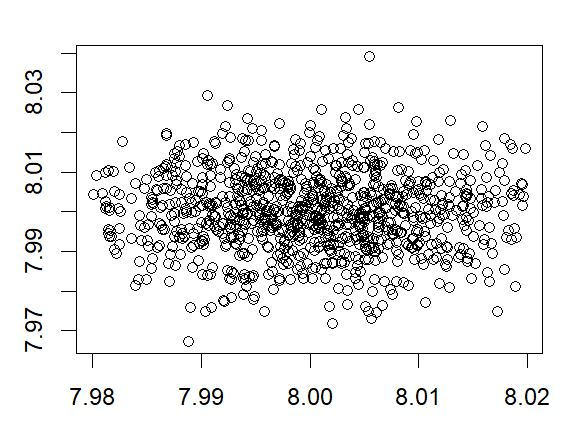
\includegraphics[width=0.5\linewidth]{images/don1.JPG}
    \caption{}
    \label{fig:enter-label}
\end{figure}

On constate que nos données n'ont pas de structure spécifique et semblent ne former qu'un seul groupe. 

La méthode de Kaufman et Rousseeuw (1990) identifie 7 clusters, ce qui, compte tenu des données, semble incohérent. Ce résultat est en accord avec la théorie exposée précédemment, car cette méthode n'est pas adaptée à des situations où un seul cluster est attendu. 
\subsection*{Méthode du Gap Statistique}

\begin{figure}[H]
    \centering
    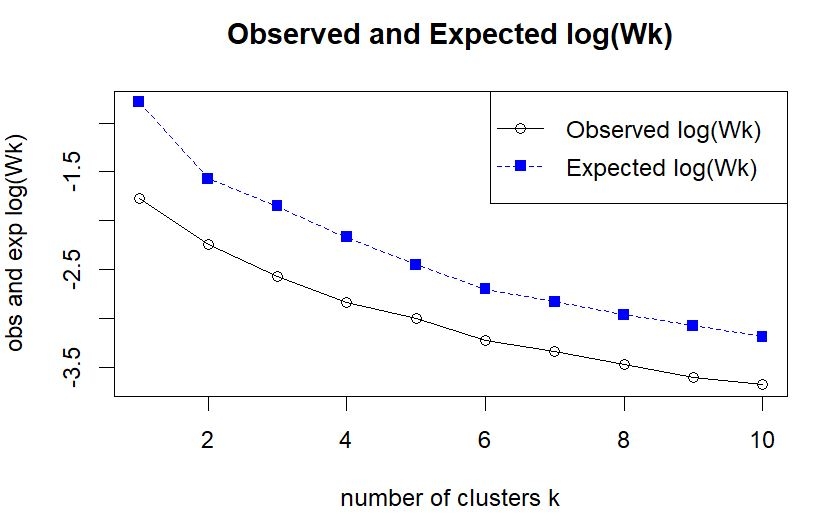
\includegraphics[width=0.5\linewidth]{images/Exp.JPG}
    \caption{}
    \label{fig:enter-label}
\end{figure}

On Constate en essayant d'observer la courbe du \(log(W_k)\) que la méthode du coude ne nous permet pas de conclure sur le nombre optimal de cluster. 

\begin{figure}[H]
    \centering
    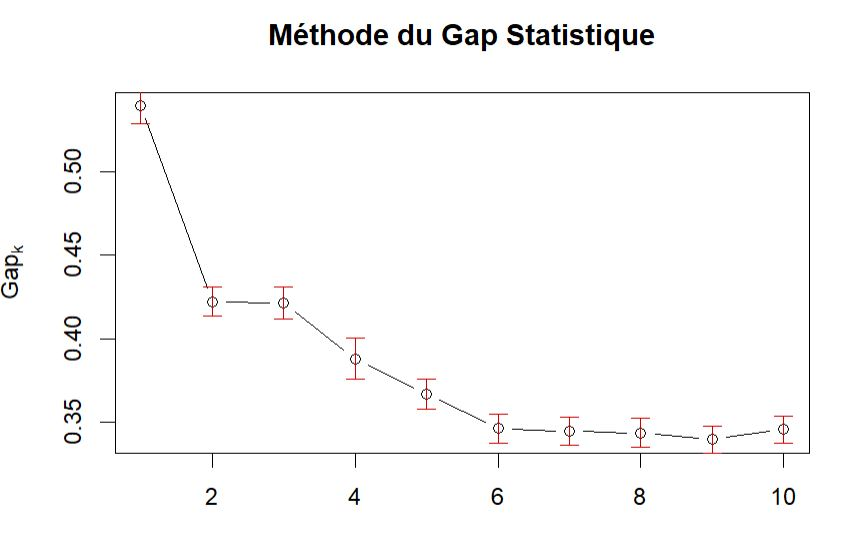
\includegraphics[width=0.5\linewidth]{images/Gaps.JPG}
    \caption{}
    \label{fig:enter-label}
\end{figure}


On constate que la méthode du Gap Statistique permet de donner de meilleurs résultats. En effet elle permet de conclure qu'il y a un seul cluster dans les données. ce qui correspond à la structure des données simulées. 

\newpage
\subsection{Données ayant trois clusters}
 Considérons maintenant un jeux de données simulé de façons à obtenir trois clusters et essayons de vérifier si la méthode du Gap Statistique permettra de trouver le même nombre de clusters.

\begin{figure}[H]
    \centering
    % 上面的大图
    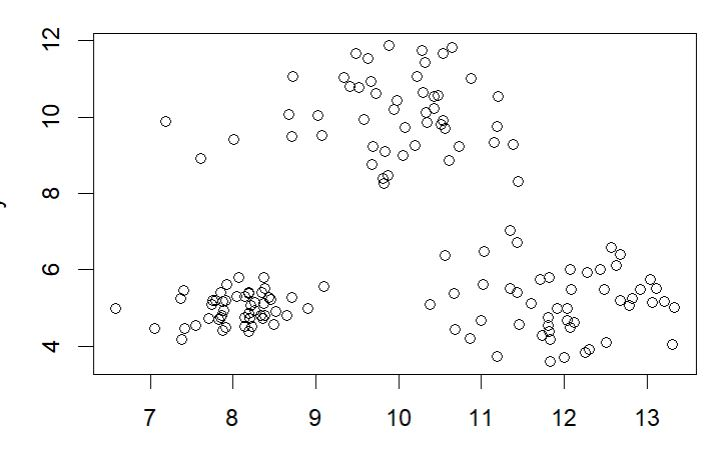
\includegraphics[width=0.7\linewidth]{images/obs2.JPG}
    \caption{}
    \label{fig:large-image}
    
    % 下面两个小图并排
    \begin{subfigure}[b]{0.45\linewidth} % 左侧子图
        \centering
        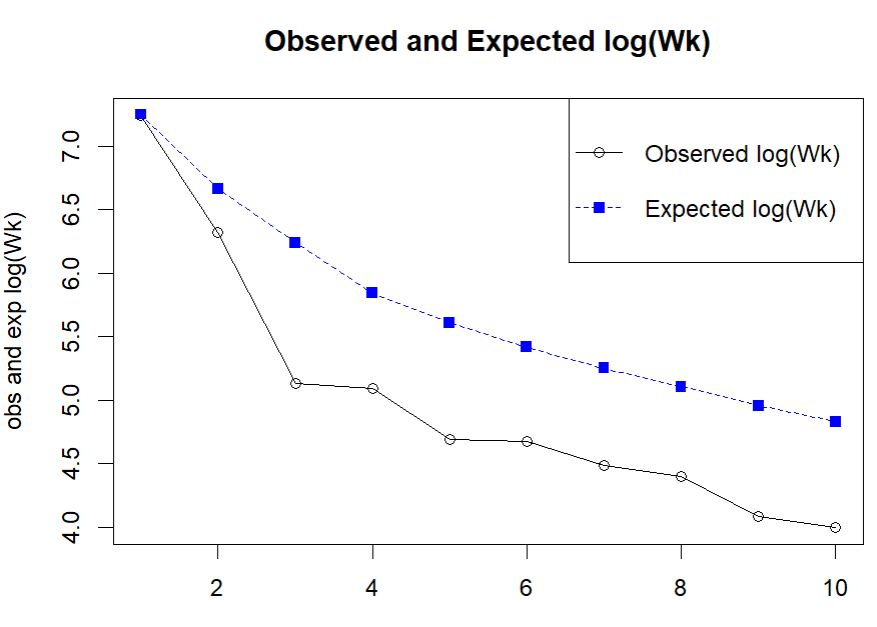
\includegraphics[width=\linewidth]{images/Exp2.JPG}
        \caption{Obs et Expected}
        \label{fig:Obs et Expected}
    \end{subfigure}
    \hspace{0.05\linewidth} % 两个子图之间的间距
    \begin{subfigure}[b]{0.47\linewidth} % 右侧子图
        \centering
        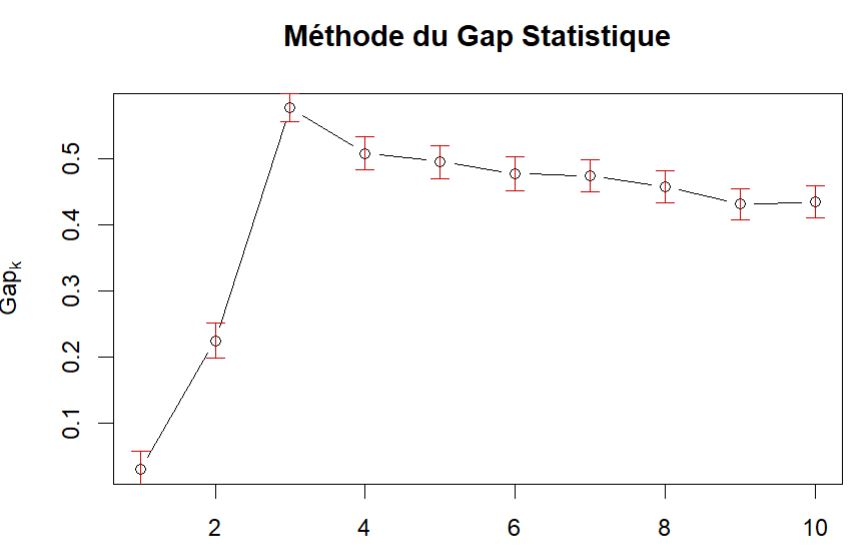
\includegraphics[width=\linewidth]{images/Gaps2.JPG}
        \caption{Gap statistique}
        \label{fig:right-small}
    \end{subfigure}
    \caption{}
    \label{fig:combined-figure}
\end{figure}

A l'aide de la règle du coude, on peut déduire que nous avons trois clusters dans notre jeux de données. De mémé, la méthode du Gap Statistique donnée par la figure (6) permet d'aboutir au même résultat. 

\newpage
\subsection{Cas d'une base de donnée réelle}

Nous allons dans cette sous section utiliser une base de données réelle. Nous avons choisis la base de données \textit{'Live'} qui contient des informations collectées auprès de vendeurs sur Facebook en Thaïlande. Les variables sélectionnées après avoir vérifié les éventuelles corrélations sont: (Le nombre total de commentaires sur la publication,Le nombre total de partages,Le nombre total de Like,Le nombre total de "Love",Le nombre total de "Wow","Haha" et de "Haha" )

En utilisant la règle du coude, on constate que le nombre de cluster optimal est entre 3 et 4 comme le montre la figure (7):

\begin{figure}[H]
    \centering
    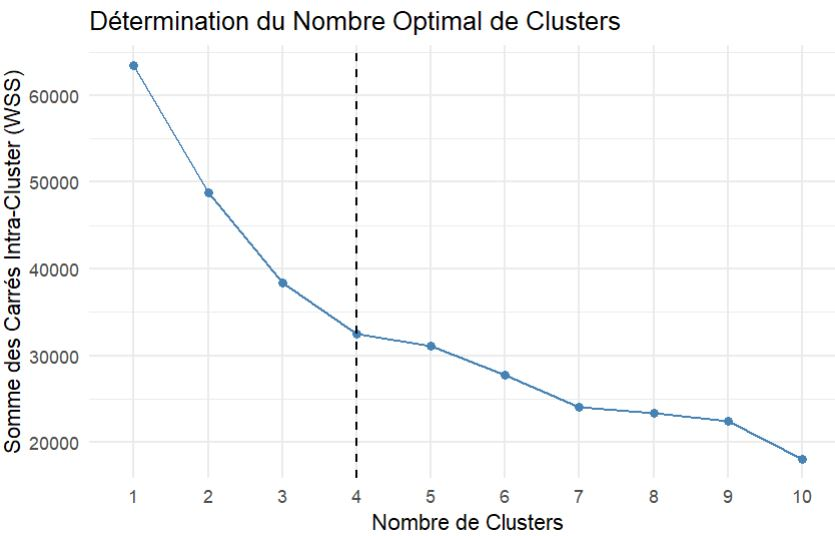
\includegraphics[width=0.8\linewidth]{images/Coude.JPG}
    \caption{}
    \label{fig:coude}
\end{figure}

En utilisant la méthode de Kaufman et Rousseeuw (1990) basée sur la statistique de la Silhouette, on obtient deux clusters avec un score optimal de 0.82.
 
En utilisant le Gap statistique, on obtient un seul cluster comme le montre la figure suivante. Ce qui semble ne pas être cohérent vu les résultats obtenus avec la méthode du coude. 

\begin{figure}[H]
    \centering
    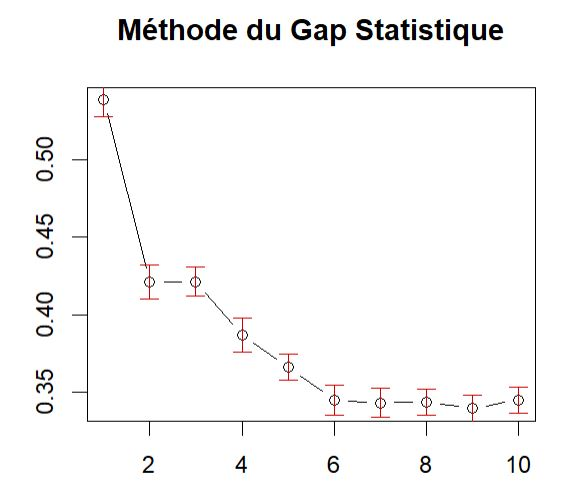
\includegraphics[width=0.6\linewidth]{images/Gap3.JPG}
    \caption{}
    \label{fig:gap3}
\end{figure}

Ce résultat, relativement imprécis, pourrait s'expliquer par deux facteurs principaux. D'une part, la méthode du Gap Statistique repose sur une hypothèse forte concernant la distribution des données, en supposant qu'elle suit une loi log-normale. D'autre part, la valeur espérée de \(log(W_k)\) est obtenue par des simulations numériques, ce qui la rend sensible au nombre de simulations effectuées ainsi qu'à la méthode employée pour générer ces données simulées.


%\part{Conclusion}
\chapter{Conclusion}

\startcontents[Conslusion]
\section*{Conclusion et Limites de la méthode du Gap Statistique}

Dans ce travail, nous avons d'abord présenté la méthode du Gap Statistique développée par Tibshirani et al. (2000), avant de l'appliquer sur deux types de données : d'une part, des données simulées dont le nombre optimal de clusters est connu, et d'autre part, une base de données réelle. Nos résultats montrent que la méthode du Gap Statistique constitue un outil puissant pour déterminer le nombre de clusters dans un jeu de données lorsque la distribution sous-jacente est inconnue.

Contrairement à d'autres méthodes couramment proposées dans la littérature, qui peuvent se révéler inefficaces en présence d'une seule composante dans les données, le Gap Statistique offre une approche robuste permettant de vérifier la nécessité ou non d'un clustering.

Cependant, cette méthode présente certaines limites. En particulier, elle peut produire des résultats erronés lorsque la distribution des données n'est pas log-normale. Dans de tels cas, des alternatives comme celle proposée par Kaufman et Rousseeuw (1990) peuvent être plus efficaces, car elles ne reposent sur aucune hypothèse spécifique concernant la distribution des données.

%----------------------------------------------------------------------------------------
%	BIBLIOGRAPHY
%----------------------------------------------------------------------------------------
\fancyhead[OL]{\textsc{Bibliographie}}
\printbibliography[
notcategory=cited,
heading=bibintoc,
title={Bibliographie}]

\end{document}
